\section{Introduction}
\label{sec:introduction}

Android's open-source nature and vast app ecosystem have fueled its widespread adoption. To regulate access to sensitive data, it uses a permission framework as a gatekeeper that lets users grant or deny each permission individually~\cite{alkindi2019android}. However, Wagner et al.\cite{ha2013android} found that only 17\% of users pay attention to permissions when installing or using apps. Once granted, permissions allow unrestricted data access, compromising user privacy\cite{alkindi2019android}. Conversely, denying permissions can lead to apps blocking not only relevant features but also unrelated ones, leaving users with no choice but to grant access.

\begin{figure}[t]
    \centering
    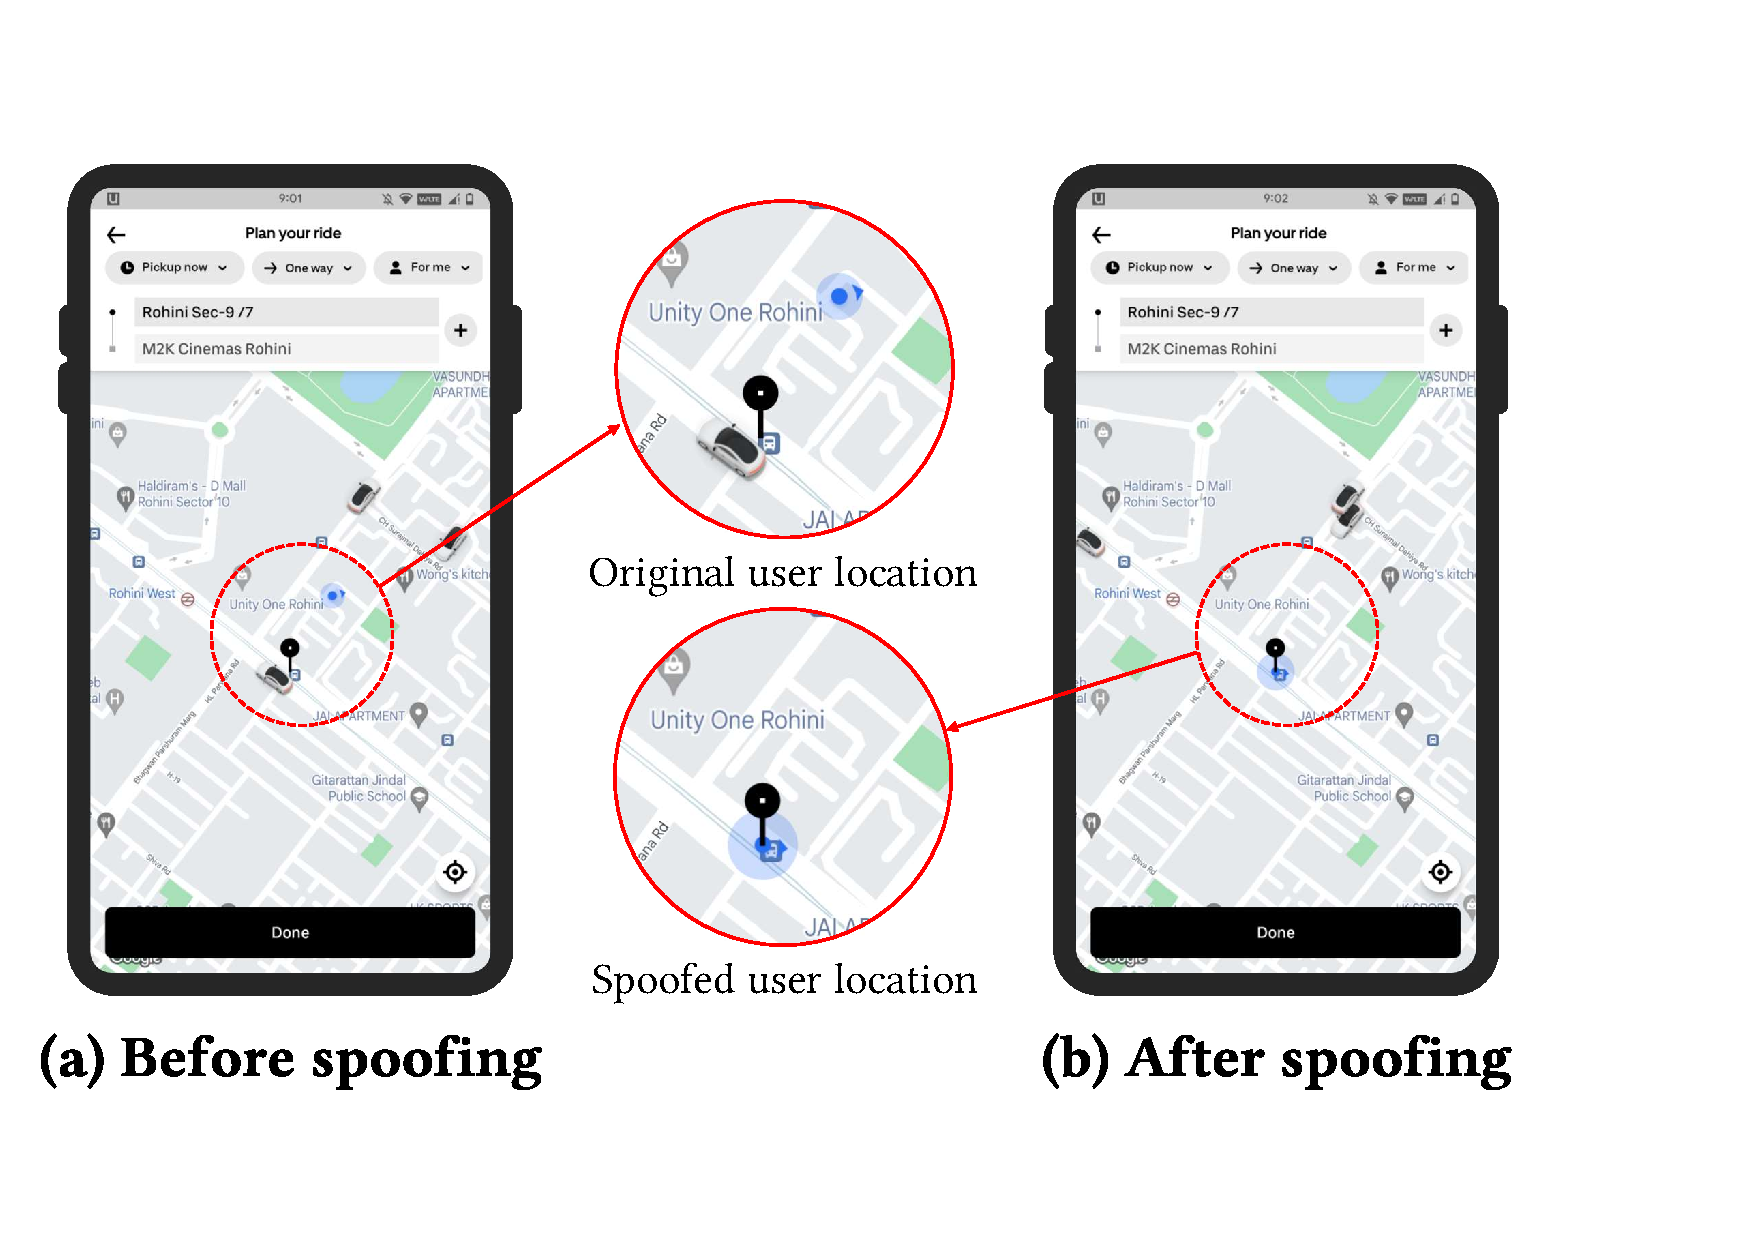
\includegraphics[width=0.75\linewidth]{Figures/Case Studies/uber_screenshots.pdf}
    \caption{Screenshots illustrating how a user can share spoofed location using \framework{} with the Uber app.}
    \label{fig:intro_case_study_uber}
\end{figure}

To protect user privacy without restricting app functionality, users could have the option to feed spoofed data to apps. Figure~\ref{fig:intro_case_study_uber} shows such a case study. In Figure~\ref{fig:intro_case_study_uber}a, Uber encourages users to share their real location, compromising privacy, even when they prefer a pinned pickup spot. Figure~\ref{fig:intro_case_study_uber}b shows how users can spoof their location, preserving privacy while still accessing Uber's cab-finding service.

Unfortunately, existing approaches for spoofing the user data involve either modifying the Android OS~\cite{smalley2013security,raval2016you,wu2017context} or rebuilding the target app binary~\cite{backes2015boxify,jeon2012dr}, which have severe limitations in terms of usability and practicality. Modifying the OS requires rooting the device which is not practical for users~\cite{zhang2015android}. Rebuilding app binary is not always successful as it can be easily detected by using Google's Play Integrity API, making the app prevent users from accessing its services~\cite{andPlayIntAPI}. 

To equip users protect their privacy, we developed \textit{\framework{}}, a comprehensive and robust data spoofing system for non-rooted Android devices. Our evaluation shows that it successfully spoofs 78.32\% of requested permissions across 70 popular apps without detection or crashes.

We further show that \framework{} can bypass continuous authentication mechanisms. Researchers have developed various such mechanisms relying on device sensor data (e.g., accelerometer)~\cite{kolokas2019gait,sun2018artificial,thang2012gait,hoang2013adaptive,shih2015flick,nohara2016personal,lu2015safeguard,jain2015exploring,nixon2016slowmo,feng2014tips,abuhamad2020autosen,amini2018deepauth,li2018using,yan2018towards,song2016eyeveri,xia2018motionhacker,hong2016mgra,hong2015waving,miguel2016interaction,zhang2016voicelive,wang2019voicepop,johnson2013secure,khamis2016gazetouchpass,zhu2013sensec,sitova2015hmog,pang2019mineauth,acien2019multilock,zhu2019riskcog,lee2017implicit}. Unlike passwords, continuous authentication runs in the background, monitoring user behavior and biometrics for identity validation. To our knowledge, \framework{} is the first to demonstrate the ineffectiveness of sensor-based authentication on Android.

\begin{table}
    {\centering
    \begin{tabular} {>{\arraybackslash\centering}m{2.5cm} >{\arraybackslash}m{9.5cm}}
        \hline
         \textbf{Use Case} & \textbf{Example(s)}\\
         \hline
         Bypassing Continuous Authentication & 
         \textbf{MGRA}~\cite{hong2016mgra} (Sec \ref{sec:continuous_authentication_mechanisms}) utilizes the accelerometer data and \textbf{VoiceLive}~\cite{zhang2016voicelive} (Sec \ref{sec:continuous_authentication_mechanisms}) utilizes the smartphone's two different microphones to authenticate users. But \framework{} proves to be capable of bypassing these authentication mechanisms by spoofing the input data. \\
         \hline
         Granting Selective User Data & 
         \textbf{Snapchat}(\hyperref[sec:sc_case_study]{Sec 5.3}) and \textbf{Truecaller}(\hyperref[sec:tc_case_study]{Sec 5.4}) requires users private data like Contacts and Messages to enable users to utilize functionalities provided by them, but this also compromises the private information. However, \framework{} enables users to grant partial data to apps that is essential.\\
         \hline
         Protection from Malicious Apps & 
         \textbf{All Good PDF Scanner} (Sec \ref{sec:malicious_apps}) was granted permissions like Storage and Camera but was detected to be uploading data on the internet in the background, hence its internet access was blocked by \framework{}. \textbf{Unique Keyboard} (Sec \ref{sec:malicious_apps}) was found to be accessing the sensor data while running in the background, therefore \framework{} fed deceived data when app is running in the background.\\
         \hline
         Side-Channel Attack Mitigation & 
         \textbf{Gyrosec}~\cite{lin2019motion} (Sec \ref{sec:side_channel_attack}) records the sensor data while running in the background, and uploads it over the internet. This was mitigated by deceiving the sensor data received by the apps.  \\
         \hline
         Unexpected Sensor Usage Detection & 
         \textbf{Facebook} (Sec \ref{sec:fb_case_study}) requested for Audio permission. But it was found (using \framework{}) to be recording the microphone data when no activity requiring microphone was being used by the user.\\
         \hline
         User Privacy Protection & 
         \textbf{Snapchat} (Sec \ref{sec:sc_case_study}) and \textbf{Truecaller} (Sec \ref{sec:tc_case_study}) provide great features to users but at the cost of sharing private information like Location, Contacts and Messages. \framework{} enables users to enjoy the provided features without compromising private information.\\
         \hline
    \end{tabular}
    }
    \caption{Various use cases of \framework{} and their respective real-world example(s)}
    \label{tab:highlights}
\end{table}

\framework{} effectively detects malicious behaviors and safeguards user data from recently banned apps. For example, it identified the "\textit{All Good PDF Scanner}" app uploading private files online and blocked its internet access without crashing or limiting its features. We also demonstrate \framework{}'s ability to detect and mitigate side-channel attacks. In our experiments, a malicious app's screen touch position prediction accuracy dropped from 81.22\% to just 5.36\% when \framework{} was used.

\framework{} not only protects against malicious apps but also enhances user privacy control. Using three real-world apps as case studies, we show how \framework{} detects privacy violations. For instance, it uncovered that the Facebook app records user audio while scrolling through posts, a behavior not indicated by Android's privacy indicator (green dot). \framework{} can also spoof audio to protect user privacy here.

A demonstration video of employing \framework{} for user data spoofing on the Facebook app is available on \href{https://www.youtube.com/watch?v=sXiGUoqFLmk}{Youtube}\footnote{https://www.youtube.com/watch?v=sXiGUoqFLmk}. Table \ref{tab:highlights} highlights various usages of \framework{} with examples.

We confirm that using \framework{} for spoofing sensitive user data results in a minimal overhead: 2.52\% increase in battery drain, 5.2 MB additional memory usage, and an average of 1.64 ms per spoofed API call. Our tests showed no noticeable performance degradation in apps.

\noindent Overall, we make the following key contributions:
\begin{itemize}[noitemsep, topsep=0pt]
\item \framework{} enables user data spoofing without rooting or modifying app binaries while maintaining minimal overhead.
\item It exposes limitations in sensor-based continuous authentication mechanisms.
\item It mitigates direct and side-channel privacy attacks from malicious apps.
\item It enhances privacy control in real-world apps like Facebook, Snapchat, Truecaller, and Uber.
\end{itemize}

The paper is structured as follows: Section~\ref{sec:motivation} presents the motivation for \framework{}. Section~\ref{sec:methodology} explains its methodology, followed by its architecture in Section~\ref{sec:architecture}. Sections~\ref{sec:mitigating_sca} and~\ref{sec:protecting_up} showcase \framework{}'s effectiveness in mitigating privacy threats and empowering users. Section~\ref{sec:results} evaluates its performance. Section~\ref{sec:related_work} reviews related work, and Section~\ref{sec:conclusion} concludes the paper.
